% !TEX TS-program = pdflatex
% !TEX encoding = UTF-8 Unicode

% This is a simple template for a LaTeX document using the "article" class.
% See "book", "report", "letter" for other types of document.

\documentclass[11pt]{article} % use larger type; default would be 10pt

\usepackage[utf8]{inputenc} % set input encoding (not needed with XeLaTeX)
\usepackage{subcaption}
%%% Examples of Article customizations
% These packages are optional, depending whether you want the features they provide.
% See the LaTeX Companion or other references for full information.

%%% PAGE DIMENSIONS
\usepackage{geometry} % to change the page dimensions
\geometry{a4paper} % or letterpaper (US) or a5paper or....
% \geometry{margin=2in} % for example, change the margins to 2 inches all round
% \geometry{landscape} % set up the page for landscape
%   read geometry.pdf for detailed page layout information

\usepackage{graphicx} % support the \includegraphics command and options

% \usepackage[parfill]{parskip} % Activate to begin paragraphs with an empty line rather than an indent

%%% PACKAGES
\usepackage{booktabs} % for much better looking tables
\usepackage{array} % for better arrays (eg matrices) in maths
\usepackage{paralist} % very flexible & customizable lists (eg. enumerate/itemize, etc.)
\usepackage{verbatim} % adds environment for commenting out blocks of text & for better verbatim
\usepackage{subfig} % make it possible to include more than one captioned figure/table in a single float
% These packages are all incorporated in the memoir class to one degree or another...

%%% HEADERS & FOOTERS
\usepackage{fancyhdr} % This should be set AFTER setting up the page geometry
\pagestyle{fancy} % options: empty , plain , fancy
\renewcommand{\headrulewidth}{0pt} % customise the layout...
\lhead{}\chead{}\rhead{}
\lfoot{}\cfoot{\thepage}\rfoot{}

%%% SECTION TITLE APPEARANCE
\usepackage{sectsty}
\allsectionsfont{\sffamily\mdseries\upshape} % (See the fntguide.pdf for font help)
% (This matches ConTeXt defaults)

%%% ToC (table of contents) APPEARANCE
\usepackage[nottoc,notlof,notlot]{tocbibind} % Put the bibliography in the ToC
\usepackage[titles,subfigure]{tocloft} % Alter the style of the Table of Contents
\renewcommand{\cftsecfont}{\rmfamily\mdseries\upshape}
\renewcommand{\cftsecpagefont}{\rmfamily\mdseries\upshape} % No bold!

% MATH
\usepackage{graphicx}
\usepackage{subfig}

\usepackage{mathtools}
\usepackage{float}
\usepackage{listings}
%%% END Article customizations

%%% The "real" document content comes below...

\title{Numerical Optimization - KETCHUP Week}
\author{Martin Simon Haugaard - CDL966}
%\date{} % Activate to display a given date or no date (if empty),
         % otherwise the current date is printed 

\begin{document}
\maketitle
\section*{Introduction}
During this course I had little focus on the Inverse Kinematic framework, only implementing stuff when explicitly tasked to, thus not doing the extra assignments. This meant that I did not have many implemented methods for testing convergence. The methods which I did have are as follows:
\begin{gather*}
\text{armijo backtracking line-search, nonlinear newton, BFGS and dogleg}
\end{gather*}
\section*{Convergence Rates}
Theoretically each of my methods should have the following cost and rate-of-convergence:
%\section*{Prove of convergence}
\begin{table}[h!]
\begin{tabular}{lllll}
Implementation & Method & cost-per-iteration & rate-of-convergence\\
\hline
armijo backtracking line-search & Steepest Descent& $O(n)$ & Q-linear &\\
nonlinear newton &Newton & $O(n^3)$ & Q-quadratic & \\
BFGS & Quasi-Newton & $O(n^2)$ & Q-super-linear & \\
dogleg & Trust-Region Method & $O(n^3)$ & Q-quadratic\\
\end{tabular}
\caption{cost-per-iteration and rate-of-convergence for methods implemented in IK framework.}
\label{table:con}
\end{table}

Observing Table~\ref{table:con} it's not trivial to see which of these methods would be the fastest to solve our Inverse Kinematic robot-arm problem. The newton method, and dogleg method (which uses newton) claim the best rate-of-convergence, but at the same time, they have the highest theoretical cost per iteration. Meanwhile the steepest descent method is fairly cheap per iteration, but only claims a linear rate-of-convergence. Lastly the BFGS method has a balance between not being the most costly per iteration, but neither having the highest convergence rate.

In order to better examine the problem, I choose to time each of the methods, randomly generating coordinates within the feasible region of the model, and testing each method once per coordinate generated. In order to minimize any outside influence, by either hardware / operation system etc. Each method was tested for each coordinate in sequence
\begin{gather*}
newton \rightarrow dogleg \rightarrow BFGS \rightarrow steepest~descent
\end{gather*}
before a new coordinate was found and the  sequence would repeat itself, thus sharing any stress there may have been during testing across all the methods, hopefully causing the stress to have equal affect on my results.

The parameters needed for each of the methods, was a matter of manually testing each of the implementations. Some would require a higher tolerance threshold than others (especially the BFGS proved difficult as its threshold had to be increased while the variables for the step-length had to be surprisingly small, and even despise my best effort BFGS still produces less than satisfying results with certain coordinates.
%Steepest Descent - Linear rate-of-convergence (Theorem 3.3)
%Newton - local rate-of-convergence quadratic (Theorem 3.5) - step length 1 (non-linear newton method is just that)
%Quasi-Newton (BFGS) - super-linear convergence rate can be attained (Theorem 3.6).
%Trust-Region Method (Dogleg) - quadratic convergence rate, as trust region can be super-linear and Newton is used. (Theorem 4.9)
%The Minimum can be determined by examining the fact that a circle with radius $\Delta$ has the following property:

\subsection*{Convergence Plots}
Below are the four converge plots that my methods produce. It's worth noting that I may have a bug in my BFGS method, as it will not alway find a good solution for any given coordinate, and in some cases its convergence error will grow exponentially. Also, the dogleg plot has had some bad coordinates removed in order to clarify its general behavior, but sadly, this method can also produce errors in rare cases.

\begin{figure}[h!]
\centering
\begin{subfigure}{.5\textwidth}
  \centering
  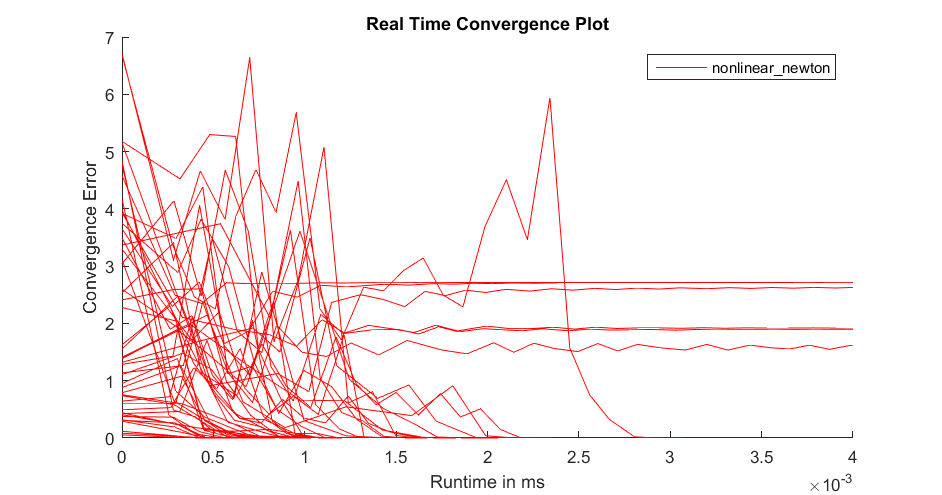
\includegraphics[width=.8\linewidth]{linear}
  \caption{nonlinear-newton}
  \label{fig:nonlinear}
\end{subfigure}%
\begin{subfigure}{.5\textwidth}
  \centering
  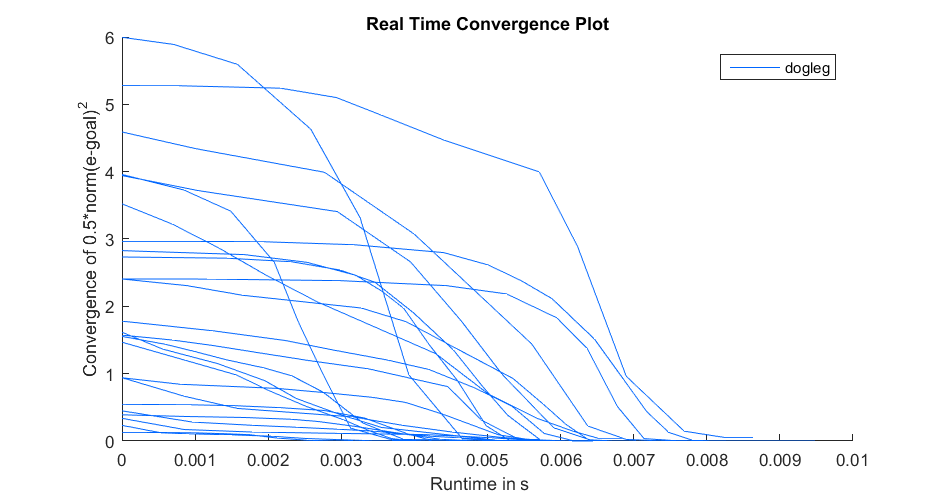
\includegraphics[width=.8\linewidth]{dogleg}
  \caption{dogleg}
  \label{fig:dogleg}
\end{subfigure}
%\caption{}
\label{fig:test}
\end{figure}

\begin{figure}[h!]
\centering
\begin{subfigure}{.5\textwidth}
\setcounter{subfigure}{2}
  \centering
  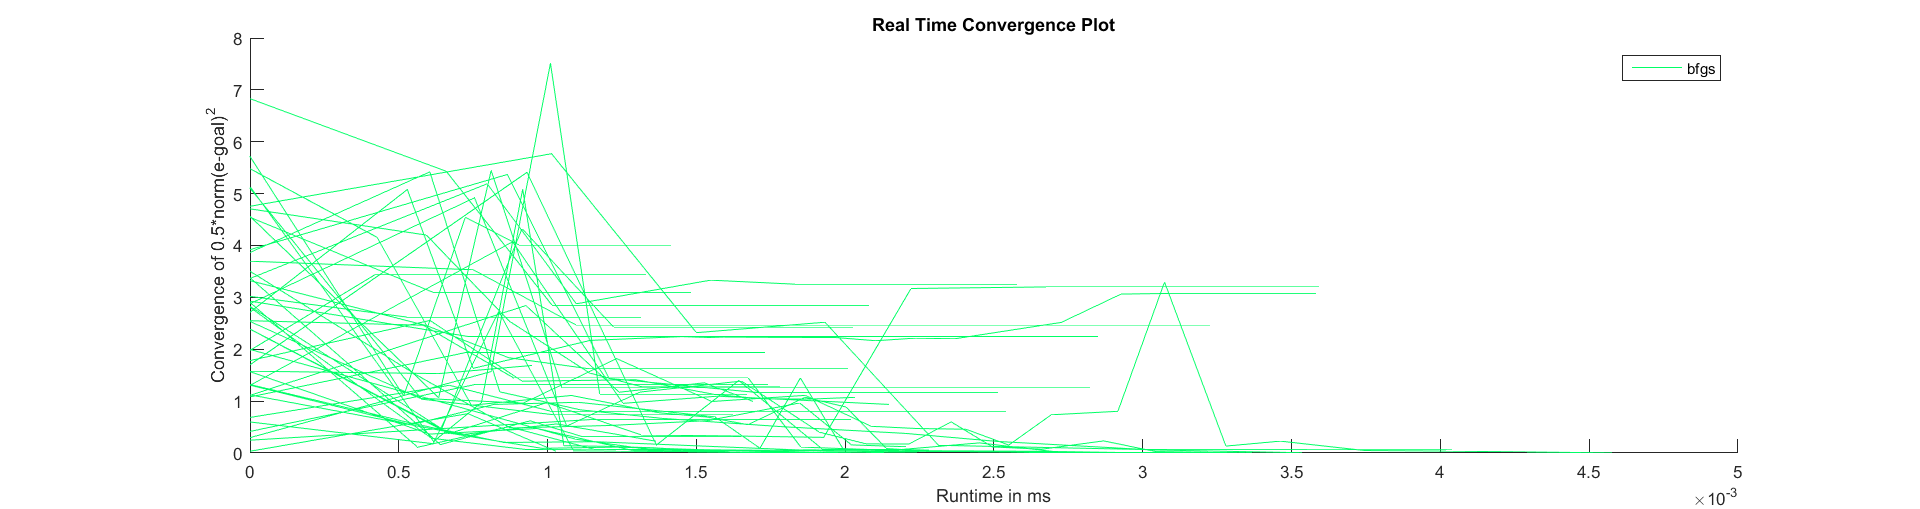
\includegraphics[width=.8\linewidth]{bfgs}
  \caption{BFGS}
  \label{fig:bfgs}
\end{subfigure}%
\begin{subfigure}{.5\textwidth}
\setcounter{subfigure}{3}
  \centering
  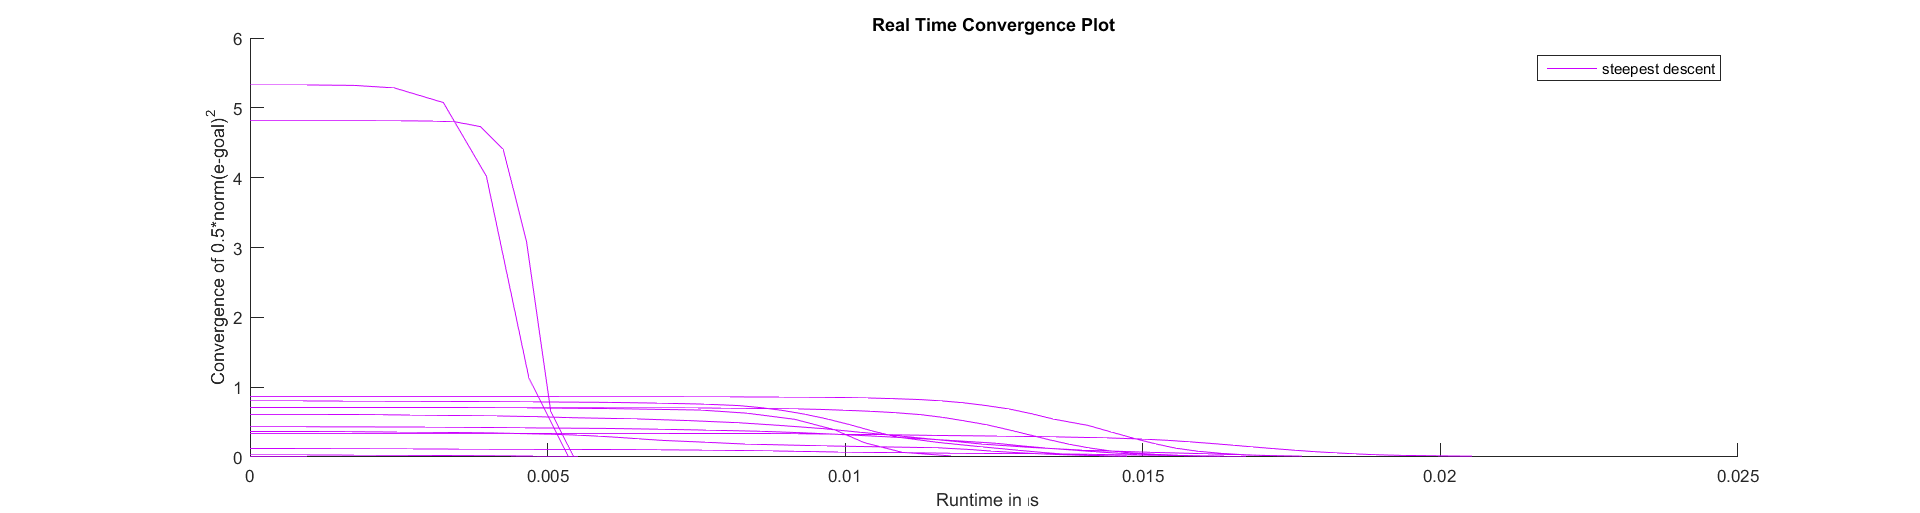
\includegraphics[width=.8\linewidth]{steepest_descent}
  \caption{Steepest Descent}
  \label{fig:dd}
\end{subfigure}
%\caption{}
\label{fig:test}
\end{figure}

Each of the above four plots uses the same measurement for convergence on the y-axis, that of
\begin{gather*}
0.5*norm(e-goal)^2
\end{gather*}
While the x-axis is elapsed time, from entering my MatLab script until leaving. On a practical note, each of these four methods would be slow for their initial plot, causing an out-lier. I assume this is due to MatLab allocating memory, as it's consistent, and very noticeable in the nonlinear-newton approach. I've chosen to skip this data-point, as it behaves just as the others, but starts roughly when the others usually end.
\newpage
Finally, in order to evaluate my four methods against each other, I've made a single plot featuring each of them on the same data coordinates:
\begin{figure}[h!]
\centering
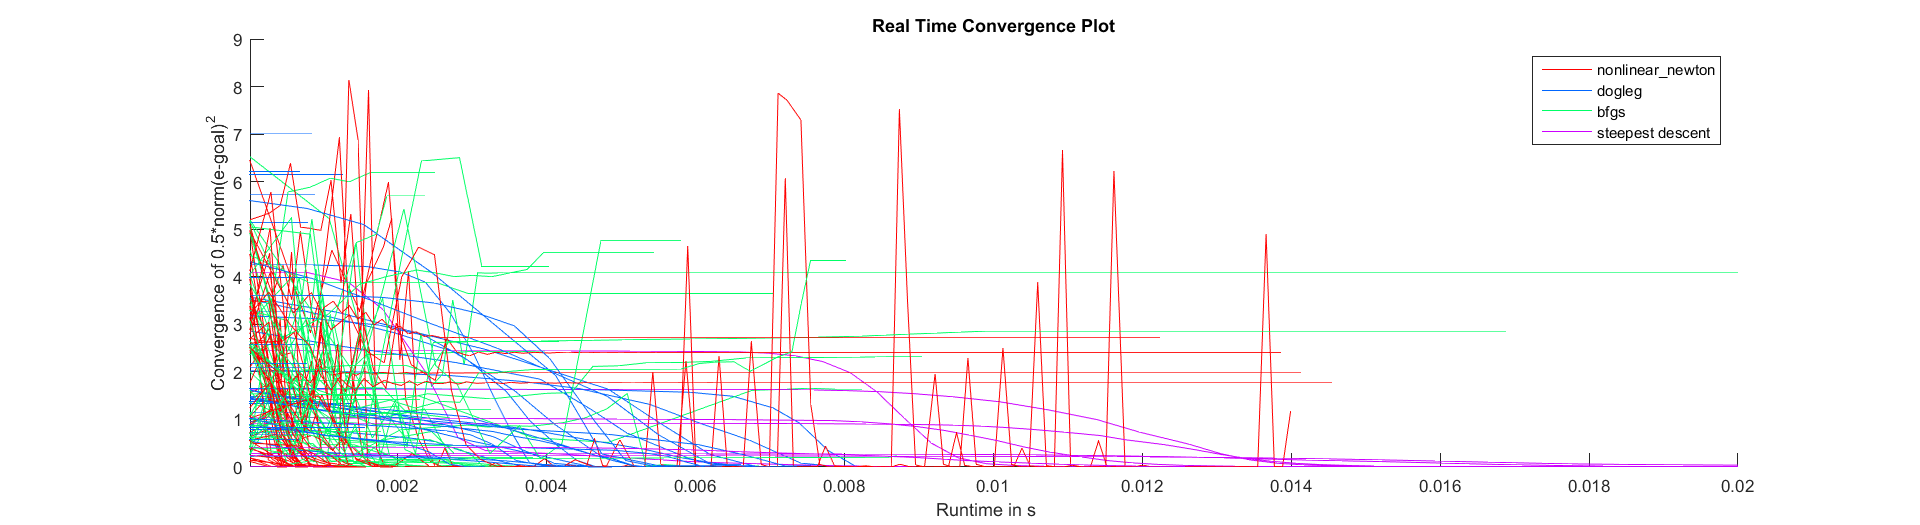
\includegraphics[width=1.2\linewidth]{overall}
\caption{}
\label{Overall convergence for all four methods.}
\end{figure}

Making conclusions from this plot can be a bit of a mess, however, it's apparent that the steepest descent method is the most robust and accurate of the four on display. It has no errors, and always seem to converge. However, it's also the slowest of the four methods to converge. 

Dogleg is a close second on both robustness and accuracy, however, depending on the initial guess it sometimes fails completely to converge, but its performance, when converging, is steady having most of its iterations take between 0.002 and 0.006s.

The nonlinear newton method is a weird one, as it is allowed to have its convergence rise as part of the implementation, and its runtime is often either very good, or very poor, making it neither very robust, accurate or efficient, as it has results varying on all fronts.

Lastly, BFGS seems to be, when converging, the best candidate if measuring speed. However, it's not very robust as is, as I expect there to be a bug in my code, causing it to sometimes gain in error instead of converging (as is the case for 8 of the 50 plots on display). However, if I were to solve the bug, I would most likely choose BFGS from among these four methods, as it seems to execute fairly well, being a mixture of rate-of-convergence and iteration cost (See Table~\ref{table:con}).

\end{document}
